\documentclass[../report.tex]{subfiles}
\def\code#1{\texttt{#1}}
\begin{document}

\onehalfspacing

\section{Hardware Design}

% TODO: Should these paragraphs be moved somewhere?
Verification across the Hardware Firmware boundary requires a system that utilizes both Hardware and Firmware in equal parts to achieve a single goal.
A secure bootloader is a program that ensures only encrypted and authenticated software is loaded onto a platform~\cite{secure-bootloader}.
In order for a bootloader to be secure it must run before any other code is executed on the platform.
Because of this, the bootloader is responsible for doing all system initialization, including hardware initialization of modules.
The bootloading process must also complete before any of the other platform code is run, meaning that program speed is important. 
The cryptographic functions of hashing and signing the authenticated software are computationally expensive and are therefore offloaded to hardware accelerators. 
All of these factors make secure boot ideal for formal verification techniques.

Verified Boot is an implementation of secure boot that has been designed by Google to run on their Chromebook laptops.
Verified Boot is the bootloader to the Chrome Operating System and verifies that all system code has been signed by Google.
Google has released both Verified Boot and Chrome OS as Open Source software, making this a viable candidate for formal verification.
While the specific hardware in each laptop is still closed source, Google has documents for extending their Verified Boot program and outlines the minimum
number of hardware modules required for security.

The hardware modules can be broken into two groups, secure storage and hardware accelerator.
Under secure storage there is an Flash memory module that provides non-volatile storage, and a Trusted Platform Module (TPM) that provides non-volatile storage that can be locked until the next boot.
Under hardware accelerators there are the cryptographic functions implementing Secure Hash Algorithm (SHA) and RSA encryption. 
The CPU accesses the hardware modules through different protocols as seen in Figure. %TODO
These interaction methods can be abstracted to Memory Mapped I/O without losing security information.

\subsection{Flash Memory}\label{flash_mem}

The Flash Memory is an amount of extra non-volatile memory connected to every Chromebook. 
The Flash Memory contains both a Read-Only section and a Read-Write section of memory.
The Read-Only section is arguably the most important piece of hardware because it is the Root of Trust of the Vboot system.
Root of Trust means that the memory within the Read-Only section is assumed to be correct.
The code within this section is the root, or base, that is responsible for verifying the rest of the Vboot process.
This code can be assumed to be untampered because it is located within the Read-Only section.
The Read-Only section is enforced by a physical screw, the Write Protect screw, which is located in the laptop.
Removing this screw removes the Root of Trust, but doing so voids the laptop's warranty.

The Read-Only memory is flashed into the laptop when the Chromebook is being built in the factory, before the Read-Only screw is added to the casing. 
The Reset Vector of the CPU points to the Read-Only flash memory, and the code located in the RO section provides information to verify the rest of the system.
In this way the RO Flash acts as the ``Root of Trust'' for the system.
In security terms, the Verified Boot process should be secure as long as the Root of Trust holds.
Inversely, if someone removes the WP screw, none of the Verified Boot security properties will hold.

Each Chrome book comes with 8 Mbs of non-volatile Flash memory~\cite{fw-summit}.
The memory is organized according to the Flashmap which I have included in the appendix.
The Flash memory is connected to the CPU by the Serial Peripheral Interface (SPI).
The SPI driver handles the protocol and provides an interface for reading multiple bytes of of memory at once.
For reasons I will mention in Section~\ref{qemu_em}, the Flash Memory will be the one Hardware piece needed for security that will not be emulated or verified.

\subsection{TPM}

The Trusted Platform Module\cite{TPM} or TPM is a general purpose cryptographic processor that is connected to a computer system for Hardware based security.
A TPM can be created by any company, but it must conform to the standards released by the Trusted Computing Group (TCG) \cite{TCG}.
The TCG has released two specifications of TPMS and they are known as TPMs version 1.2 and 2.0.
For the scope of this project we will be looking at the TPM 1.2 specification.
The TPM specification outlines the commands, structures, and interface for the system.
The TPM commands describe the full functionality of the system by describing each command the main CPU can request.
The TPM structures describe what data structures can be passed back and forth from the CPU to the TPM, as well as what information the TPM can hold within.
The TPM interface describes the registers that are exposed to the CPU and how they should be used to send data back and forth.

\begin{figure}
  \centering
\begin{subfigure}{.4\textwidth}
  \centering
  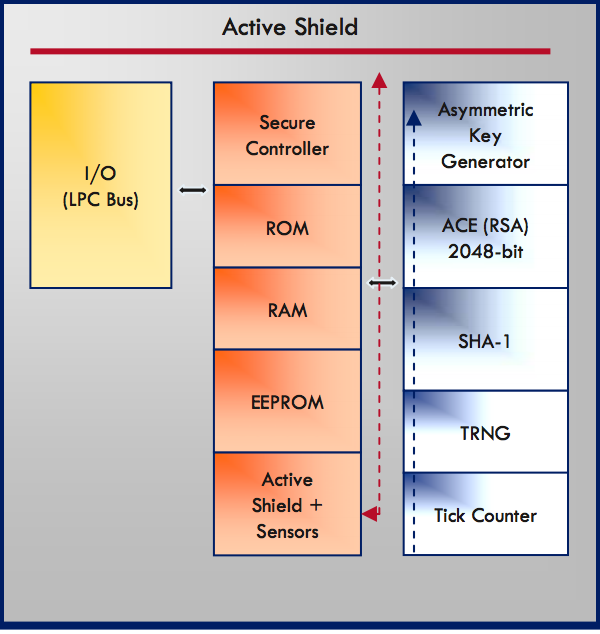
\includegraphics[width=1.0\linewidth]{tpm_hw.png}
\end{subfigure}
\begin{subfigure}{.40\textwidth}
  \centering
  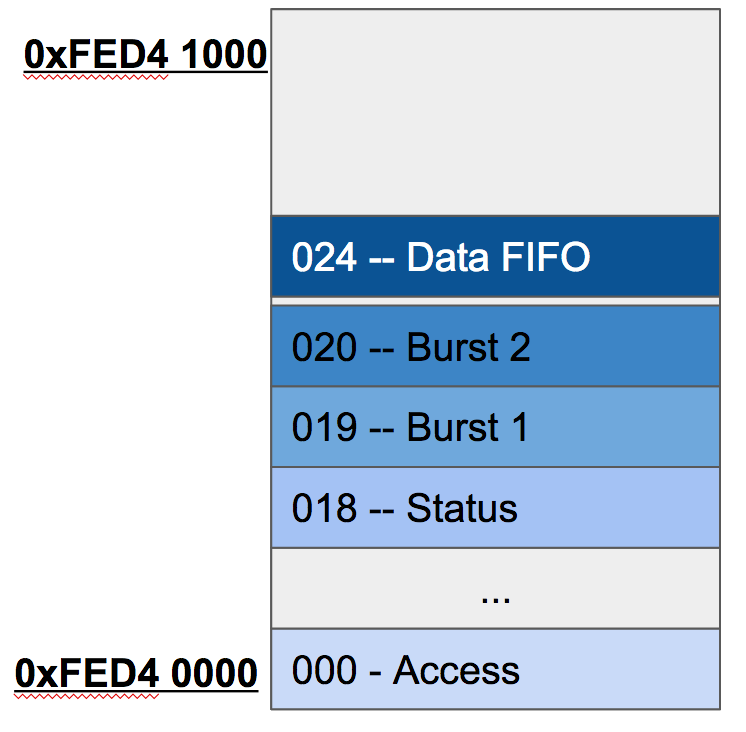
\includegraphics[width=1.0\linewidth]{tpm_regs.png}
\end{subfigure}
\caption{On the left we can see the registers of the TPM that are accessed by the CPU~. On the right we can see a HW block diagram of the TPM itself\cite{tpm-slides}.}
\label{fig:tpm_hw}
\end{figure}

We can see from Figure~\ref{fig:tpm_hw} that the TPM includes many cryptographic engines. 
Additionally it contains its own storage (volatile and non-volatile), that can be accessed from the main CPU in specific ways.
For the purpose of this report, the TPM is used as a module that can securely store keys and measurements made by the bootloader.

\subsubsection{TPM Interface}

The CPU communicates to the TPM by reading and writing specific memory addresses.
These addresses allow the CPU to send multi-byte commands to the TPM and receive multi-byte responses, even though a single byte is read or written at a time.
I describe the registers below.

\begin{itemize}
    \item \code{Status} --- This register allows the CPU to know what state the TPM is currently in. Specifically, there are bits for  if the TPM is currently accepting or sending a command, or if the TPM is busy. Specific values can be written to this register to tell the TPM to start accepting a command, or to run a command that has been sent.
    \item \code{Burst} --- Reading this register lets the CPU know how many bytes can be read (if sending a command) or written (if receiving a command) at a single time.
    \item \code{Data} --- Reading this register reads one byte of data from the TPM~. Writing this register sends one byte of data to the TPM~.
\end{itemize}

% TODO: Should this be itemized or put into a graphic?
Sending a command serially to the TPM works in the following way.
First, the \code{Command\_Start} value is written to \code{Status}.
Second, the \code{Burst} register is read to see how many bytes the TPM can accept.
Next, the Data register is written to up to \code{Burst} times, until the command has been sent.
If the command is longer then \code{Burst} amount, \code{Burst} can be polled again until it becomes non-zero.
Finally, the \code{Command\_Go} value is written to \code{Status} and \code{Status} is polled until the TPM says that it has finished processing the command.

Receiving a command follows the process above, except that \code{Data} is read instead of written to.

\subsubsection{Platform Configuration Registers}

\begin{figure}
  \centering
  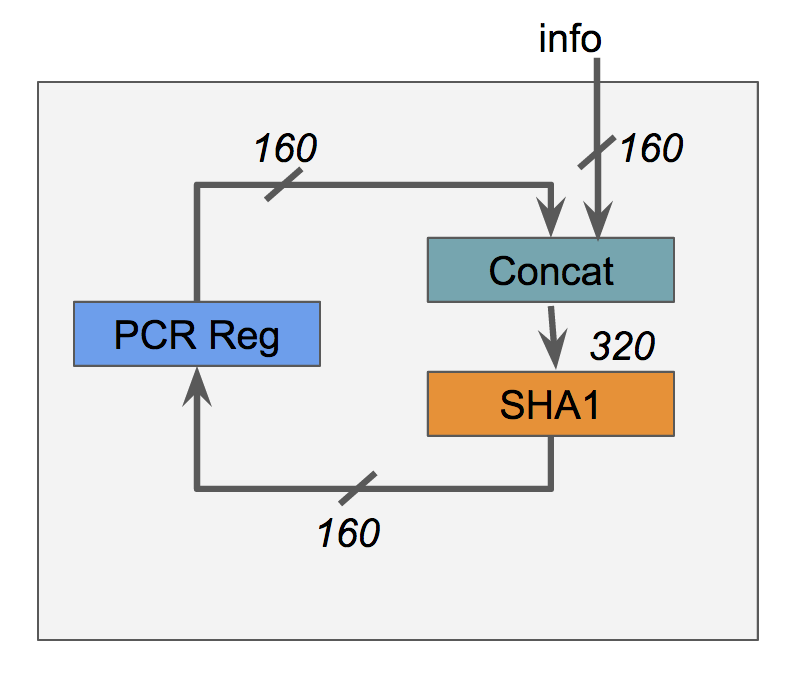
\includegraphics[width=0.4\linewidth]{pcr_alg.png}
  \caption{PCR extend Hardware Diagram}
  \label{fig:pcr_alg}
\end{figure}

Now that it is understood how commands are passed to and from the TPM, we can discuss the commands used by Google's Vboot.
There are three commands that deal with the TPM's Platform Configuration Registers or PCRs.
Under specification 1.2, a TPM is required to have 21 PCRS, each PCR is 20 bytes long and they are stored in the TPM's non-volatile storage.
The goal of these registers is to store measurements of the system state in a secure way. 
PCRs are secure storage because they cannot be written to directly, they are either extended or reset. 
PCRs are extended by concatenating the current the current PCR value with the input, and then storing the SHA1 hash of the result. 
The hardware diagram of this process can be seen in Figure~\ref{fig:pcr_alg}.
Resetting the PCR changes the value to all zeros, although the PCRs used by VBoot have the reset functionality disabled.
PCRs can also be locked, meaning that they are then unable to be extended or reset for the remainder of the system's power cycle.

Because the PCRs store a SHA1 Hash, they are useful for taking the measurement of a system.  
Hashing is a one way cryptographic function that is used to protect the integrity of a message.
We can think of a hash as the fingerprint of a message, because it takes an arbitrary length of data and outputs a fixed length (20 bytes).
The PCRs are iteratively extended with measurements of the system, for example, the hash of the Read Only Firmware, then the hash of the Read Write Firmware, and then the hash of the Kernel.
The final result will be identical each time if and only if there were no changes in each of the things being measured.
By the definition of hashing, it is difficult also to find a fake configuration of the system that will hash to the same value as a correct configuration, meaning that if the hashes are equal it is reasonable to assume that the system is unchanged. 
% TODO: ^^^ wording is a little wonky, and might be moved

\subsection{SHA}
\subsection{RSA}

\subsection{QEMU Emulation}\label{qemu_em}

\begin{figure}
  \centering
  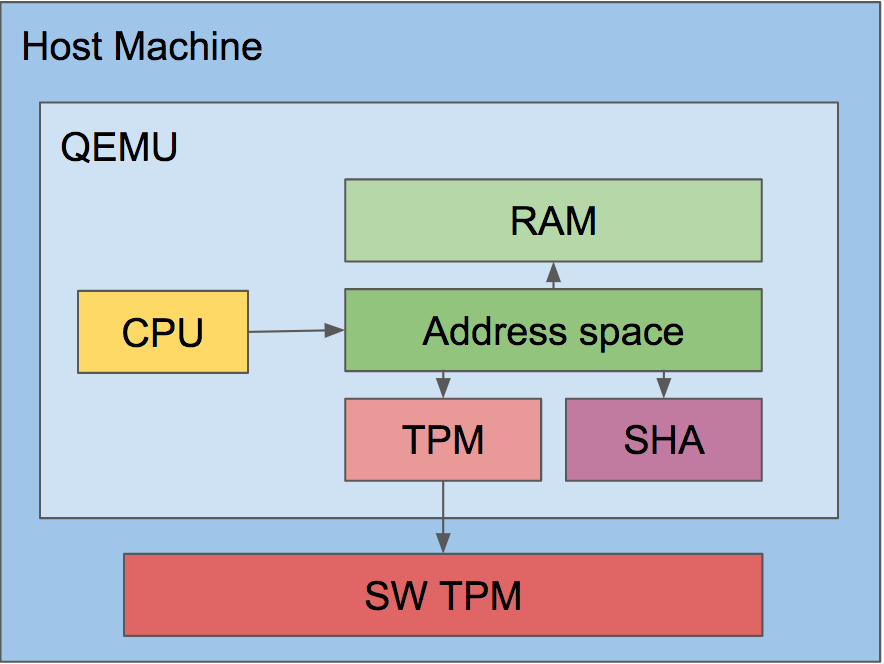
\includegraphics[width=0.4\linewidth]{qemu_layout.png}
  \caption{The QEMU layout. We can see here how the CPU and other hardware modules write RAM, and how some QEMU modules are interfaces to external software libraries.}
  \label{fig:qemu_layout}
\end{figure}

QEMU is an open source full machine emulator~\cite{qemu-site}.
For this project it is used to emulate a 32 bit i386 CPU with a Memory Mapped TPM and SHA module.
To run code, I am relying on QEMU's ability to boot any image that starts with a defined multi-boot header~\cite{multiboot}.
QEMU then supplies its own bootloader, which is responsible for initializing RAM, putting the processor in 32 bit mode, and loading the image off of disk.
As we will see in Section~\ref{coreboot}, for Chromebook this job is normally taken care of by Coreboot, but for the purposes of this report it was easier to use QEMU's built-in bootloader.

The QEMU code (included in the appendix and the github link), was based off of a project developed for Open Source at Princeton by me and Lance Goodridge.
The Open Source project allowed students to build their own Operating System from scratch and develop it within QEMU\@.
The Open Source project was repurposed by this thesis for its well-organized Makefile, linker script, and multi-boot header.
These tools allowed me to create and compile a standalone C file that could hook into the Vboot repository and run Google's Verified Boot within QEMU's virtualized Hardware.

The QEMU emulator was modified to add a TPM and a SHA module, but as mentioned in Section~\ref{flash_mem} it does not include the Flash Memory.
While the Flash Memory is important as a Root of Trust in the System, its purpose is very simple.
Its main function is to provide read-only storage, and this is not a property that is difficult to be checked.
Instead of adding Flash Memory to the QEMU emulation, I load the Vboot code in with the image using the linker script. %TODO link to Linker script
The linker script loads in different sections that would correspond to the Flash Memory, and these sections are accessed normally in RAM instead.

% SW TPM library -- used by IBM
% implements all of the TCG standards
% Run in userspace, but passed through to be accessed by registers
% I implemented a driver, but it is very similar to the one used by coreboot

% TODO: Get the SHA working
% Using my own SHA implementation, close to the one used by coreboot

\end{document}
